\documentclass{article}

% if you need to pass options to natbib, use, e.g.:
%     \PassOptionsToPackage{numbers, compress}{natbib}
% before loading neurips_2024


% ready for submission
\usepackage[preprint]{main}


% to compile a preprint version, e.g., for submission to arxiv, add add the
% [preprint] option:
%     \usepackage[preprint]{neurips_2024}


% to compile a camera-ready version, add the [final] option, e.g.:
%     \usepackage[final]{neurips_2024}


% to avoid loading the natbib package, add option nonatbib:
%    \usepackage[nonatbib]{neurips_2024}


\usepackage[utf8]{inputenc} % allow utf-8 input
\usepackage[T1]{fontenc}    % use 8-bit T1 fonts
\usepackage{url}            % simple URL typesetting
\usepackage{booktabs}       % professional-quality tables
\usepackage{amsfonts}       % blackboard math symbols
\usepackage{nicefrac}       % compact symbols for 1/2, etc.
\usepackage{microtype}      % microtypography
\usepackage{xcolor}         % colors
\usepackage{graphicx}	%image
\usepackage{amsmath, nccmath}	%align
\usepackage{tikz}
\usepackage[fleqn,tbtags]{mathtools}
\usepackage{cancel}
\usepackage[mathscr]{euscript}
\usepackage{tabto}
\usepackage{mathtools}

\DeclarePairedDelimiterX{\infdivx}[2]{(}{)}{%
  #1\;\delimsize\|\;#2%
}
\newcommand{\infdiv}{D_{KL}\infdivx}

% https://www.overleaf.com/read/wzwnrbbwrvyx
% https://tex.stackexchange.com/questions/162207/algorithm2e-comment-style
% https://tex.stackexchange.com/questions/298339/how-to-insert-a-continue-in-while-command-of-algorithm2e
% https://tex.stackexchange.com/questions/195991/aligning-in-and-out-text-for-algorithms
% https://tex.stackexchange.com/questions/155542/algorithm-write-if-then-return-or-else-return-in-one-line
\usepackage[linesnumbered,ruled,vlined]{algorithm2e}

% https://tex.stackexchange.com/questions/200730/how-to-have-the-algorithmicx-comment-symbol-in-algorithm2e
\SetKwComment{Comment}{$\triangleright$\ }{}
% \newcommand\mycommfont[1]{\footnotesize\ttfamily\textcolor{black}{#1}}
% \SetCommentSty{mycommfont}

\SetKwInput{KwInput}{Input}                % Set the Input
\SetKwInput{KwOutput}{Output}              % set the Output

\SetKw{Andd}{and} % `\And` already exists
\SetKw{Break}{break}
\SetKw{Continue}{continue}
\SetKw{Return}{return}

% https://english.stackexchange.com/questions/338/when-is-l-doubled

% \newcommand{\all}{\textbf{all}~}

\newcommand{\both}{\textbf{both}~}
    \newcommand{\andd}{\textbf{and}~}

\newcommand{\butalso}{\textbf{but also~}}
    \newcommand{\notonly}{\textbf{not only~}}

\newcommand{\cf}{cf.~}

\newcommand{\eg}{e.g.~}
\newcommand{\either}{\textbf{either~}}
    \newcommand{\orr}{\textbf{or}~}
% \newcommand{\every}{\textbf{every~}}

\newcommand{\first}{\textbf{Firstly},~}
    \newcommand{\second}{\textbf{Secondly},~}
    \newcommand{\third}{\textbf{Third},~}
    \newcommand{\fourth}{\textbf{Fourth},~}
    \newcommand{\final}{\textbf{Finally},~}
    \newcommand{\last}{\textbf{Lastly},~}

% \newcommand{\from}{\textbf{from}~}
%     \newcommand{\tob}{\textbf{to}~}

% \newcommand{\never}{\textbf{never}~}
% \newcommand{\no}{\textbf{no}}
\newcommand{\nott}{\textbf{not}~}

\newcommand{\ie}{i.e.~}
\newcommand{\incl}{incl.~} % https://dictionary.cambridge.org/dictionary/english/incl
\newcommand{\iiddot}{i.i.d}
% \newcommand{\iid}{\iiddot~} % many tildes may cause compile error, eg in `~\iid`
\newcommand{\st}{s.t.~}
\newcommand{\vs}{vs.~}

\newcommand{\orrr}{\textbf{or}~}

\newcommand{\wrt}{with respect to~}

% https://tex.stackexchange.com/questions/57152/how-to-draw-graphs-in-latex
% https://tex.stackexchange.com/questions/300098/draw-a-node-as-a-square-with-tikz
% https://tex.stackexchange.com/questions/350049/tikz-pgfplots-how-to-make-tikzpcture-fit-the-parent-figure-subfigure-float-envi/
% https://rmwu.github.io/tutorial/latex/2019/11/21/positioning/
% https://texample.net/tikz/examples/
\usepackage{tikz}
\usetikzlibrary{positioning, shapes.geometric, backgrounds}
% \usetikzlibrary{positioning, shapes, shadows, arrows}

% https://tex.stackexchange.com/questions/5461/is-it-possible-to-change-the-size-of-an-arrowhead-in-tikz-pgf/161238#161238
% https://tex.stackexchange.com/questions/409881/self-loop-arrowhead-different-cannot-change
% https://github.com/pgf-tikz/pgf/issues/1008
    % [>={Arrowtype}] this means "make all arrows {ArrowType}" and you supply this to generic style settings.
    % [-{Arrowtype}] this means "put an end arrow head {ArrowType}" and you supply this style to paths and edges
\usetikzlibrary{arrows.meta}

% https://tex.stackexchange.com/questions/13625/subcaption-vs-subfig-best-package-for-referencing-a-subfigure
% https://tex.stackexchange.com/questions/333249/controlling-subfigure-captions-and-subfigure-placement
% https://tex.stackexchange.com/questions/13150/subfigures-with-tikz-on-the-same-line
% http://www.peteryu.ca/tutorials/publishing/latex_captions
% \usepackage{subfigure} % clash with `subcaption`
% \usepackage{subfig}
\usepackage{subcaption}

% https://tex.stackexchange.com/questions/110513/unknown-graphics-extension-1-png
\usepackage{grffile}

% https://tex.stackexchange.com/questions/8532/is-eps-or-pdf-the-preferred-figure-format-when-typesetting-in-latex
% https://tex.stackexchange.com/questions/45498/choosing-whether-to-include-pdf-or-png-in-pdflatex
% https://www.overleaf.com/learn/latex/Managing_images
% https://www.overleaf.com/learn/how-to/Why_do_I_keep_getting_the_compile_timeout_error_message%3F
\usepackage{graphicx} % Allows including images
\DeclareGraphicsExtensions{.pdf,.jpeg,.png,.jpg}

% https://tex.stackexchange.com/questions/50070/landscape-figure-in-latex
% https://tex.stackexchange.com/questions/37600/how-to-rotate-a-group-of-figures-subfigure
% https://tex.stackexchange.com/questions/471472/how-to-make-figures-appear-landscape-properly
% https://tex.stackexchange.com/questions/438798/how-to-get-landscape-float-with-correct-numbering
% https://tex.stackexchange.com/questions/159988/sidewaysfigure-and-landscape
\usepackage{rotating}

% https://www.overleaf.com/learn/latex/wrapping_text_around_figures
% https://tex.stackexchange.com/questions/31764/white-space-under-wrapfigure-caption
\usepackage{wrapfig}

% https://tex.stackexchange.com/questions/15971/bibliography-with-page-numbers
% \usepackage[hidelinks, bookmarksnumbered]{hyperref}
\usepackage[hidelinks, bookmarksnumbered, backref=page]{hyperref}
\renewcommand*{\backref}[1]{}
\renewcommand*{\backrefalt}[4]{
  \ifcase #1 (Broken backref)
  \or        (page~#2)
  \else      (pages~#2)
  \fi
}

\hypersetup{
  colorlinks   = true,
  urlcolor     = blue,
  linkcolor    = blue,
  citecolor   = blue
}

\usepackage{url}            % simple URL typesetting

% https://tex.stackexchange.com/questions/36175/what-do-newcommand-renewcommand-and-providecommand-do-and-how-do-they-differ
% https://tex.stackexchange.com/questions/163280/underbar-changing-the-style-of-font-but-bar-not-why

% https://tex.stackexchange.com/questions/341717/smaller-font-for-subscript-within-subscript-in-math-mode
\usepackage{scalerel}
\usepackage{amsmath}
\usepackage{amsthm}
\usepackage{amssymb}
\usepackage{amsfonts}       % blackboard math symbols
\usepackage{mathtools}
\usepackage{cancel}
\usepackage{bbm} % for `\mathbbm{b}`

% https://tex.stackexchange.com/questions/479/lowercase-mathcal
\usepackage{dutchcal}

% https://tex.stackexchange.com/questions/118173/how-to-write-ceil-and-floor-in-latex
\usepackage{mathtools}
\DeclarePairedDelimiter\ceil{\lceil}{\rceil}
\DeclarePairedDelimiter\floor{\lfloor}{\rfloor}

% Math operator macros %%%%%%%%%%%%%%%%%%%%%%%%%%%%%%%%%%%%%%%%%%%%%%%%%%%%%%%%%
\newcommand{\abs}[1]{\left|#1\right|}
\newcommand{\clip}{\mathrm{clip}}
\newcommand{\cov}[1]{\mathrm{Cov}(#1)}
\newcommand{\diag}{\mathrm{diag}}

\newcommand{\E}[2]{\mathbb{E}_{#1} \left[ #2 \right]} % expectation

\newcommand{\interior}[1]{\mathrm{interior}(#1)}

\newcommand{\norm}[1]{\|#1\|} % for ordinary vectors
\newcommand{\normm}[1]{\left\|#1\right\|}
\newcommand{\nullspace}{\mathrm{Null}}

\newcommand{\partdiff}[1]{\frac{\partial}{\partial #1}}
\newcommand{\partdiffb}[2]{\frac{\partial #2}{\partial #1}}

\newcommand{\rank}{\mathrm{rank}}

\newcommand{\ud}{\mathrm{d}}

\newcommand{\prob}[1]{\mathrm{Pr}\{#1\}}

\newcommand{\realset}{\mathbb{R}}
\newcommand{\real}[1]{\mathbb{R}^{#1}}
\newcommand{\integer}[1]{\mathbb{Z}^{#1}}
\newcommand{\naturall}[1]{\mathbb{N}^{#1}}

\newcommand{\set}[1]{\left\{ #1 \right\}}
\newcommand{\setname}[1]{\mathcal{#1}}
\newcommand{\setsize}[1]{|\mathcal{#1}|}
\newcommand{\setsizesubt}[1]{|\mathcal{#1}_t|}
\newcommand{\setsizesubx}[2]{|\mathcal{#1}_{#2}|}

% http://statweb.stanford.edu/~owen/courses/363/scribe_template.tex
\newcommand{\simiid}{\stackrel{\mathrm{iid}}{\sim}}

% https://tex.stackexchange.com/questions/111544/what-is-the-capital-greek-letter-for-tau
\newcommand{\Tau}{\mathrm{T}}
\newcommand{\trace}{\mathrm{trace}}
\newcommand{\var}{\mathrm{var}}

\newcommand{\spanspace}{\mathrm{span}}

\newcommand{\eqset}{\mathrel{\overset{\makebox[0pt]{\mbox{\normalfont\tiny\sffamily set}}}{=}}}

% https://tex.stackexchange.com/questions/4216/how-to-typeset-correctly
% \newcommand{\eqdef}{\mathrel{\overset{\makebox[0pt]{\mbox{\normalfont\tiny\sffamily def}}}{=}}}
\newcommand{\eqdef}{\coloneqq}
\newcommand{\eqdefr}{\eqqcolon}

\newcommand{\widebar}[1]{\overline{#1}}
\DeclareMathOperator*{\argmin}{\arg\!\min}
\DeclareMathOperator*{\argmax}{\arg\!\max}
\renewcommand\qedsymbol{$\blacksquare$}

% `\mathbf{}` does not work for eg \hat{\mat{}}
\newcommand{\vecb}[1]{\boldsymbol{#1}}
\newcommand{\mat}[1]{\boldsymbol{#1}}

% https://tex.stackexchange.com/questions/2607/spacing-around-left-and-right/
\let\originalleft\left
\let\originalright\right
\renewcommand{\left}{\mathopen{}\mathclose\bgroup\originalleft}
\renewcommand{\right}{\aftergroup\egroup\originalright}

\newtheorem{theorem}{Theorem}[section]
\newtheorem{corollary}{Corollary}[theorem]
\newtheorem{definition}{Definition}[section]
\newtheorem{lemma}{Lemma}[section]
\newtheorem{proposition}{Proposition}[section]
\newtheorem{assumption}{Assumption}[section]
\newtheorem{remark}{Remark}[section]

% MDP special states and actions %%%%%%%%%%%%%%%%%%%%%%%%%%%%%%%%%%%%%%%%%%%%%%%
\newcommand{\szrat}{s_{\mathrm{zrat}}} % zrat: zero reward absorbing terminal
\newcommand{\azrat}{a_{\mathrm{zrat}}}
\newcommand{\pzrat}{p_{\mathrm{zrat}}}
\newcommand{\rzrat}{r_{\mathrm{zrat}}}
\newcommand{\isdzrat}{\isd_{\mathrm{zrat}}}
\newcommand{\ssetzrat}{ \setname{S}_{\mathrm{zrat}}^+ }
\newcommand{\asetzrat}{ \setname{A}_{\mathrm{zrat}}^+ }

\newcommand{\sreset}{s_{\mathrm{rst}}}
\newcommand{\areset}{a_{\mathrm{rst}}}
\newcommand{\preset}{p_{\mathrm{rst}}}
\newcommand{\rreset}{r_{\mathrm{rst}}}
\newcommand{\isdreset}{\isd_{\mathrm{rst}}}
\newcommand{\ssetreset}{ \setname{S}_{\mathrm{rst}}^+ }
\newcommand{\asetreset}{ \setname{A}_{\mathrm{rst}}^+ }

\newcommand{\sref}{s_{\mathrm{ref}}}
\newcommand{\srefcand}{\tilde{s}_{\mathrm{ref}}} % sref candidate

\newcommand{\aref}{a_{\mathrm{ref}}}

\newcommand{\strans}{s_{\mathrm{tr}}}
\newcommand{\srecur}{s_{\mathrm{re}}}

\newcommand{\strrv}{S_{\mathrm{tr}}} % random variable
\newcommand{\srerv}{S_{\mathrm{re}}} % random variable

% MDP matrices and vectors %%%%%%%%%%%%%%%%%%%%%%%%%%%%%%%%%%%%%%%%%%%%%%%%%%%%%
% https://tex.stackexchange.com/questions/352993/adjusting-subscript-distance-by-redefining-command
\newcommand{\diagpts}{\mat{D}_{\!\!p^t}^{\!\frac{1}{2}}}
\newcommand{\diagpt}{\mat{D}_{\!\!p{^{t}}}}
\newcommand{\diagpstar}{\mat{D}_{\!\!\vecb{p}^{\!\star}}}
\newcommand{\diagptilde}{\mat{D}_{\!\tilde{\vecb{p}}}}
\newcommand{\diagptildesqrt}{ \mat{D}_{\!\tilde{\vecb{p}}}^{\!\frac{1}{2}} }
\newcommand{\diagsvd}{\mat{D}_{\!\!\sigma}}
\newcommand{\diagsvds}{\mat{D}_{\!\!\sigma}^2}
\newcommand{\diageig}{\mat{D}_{\!\!\mu}}

\newcommand{\ppimat}{\mat{P}_{\!\!\pi}} % one-step transition matrix under pi
\newcommand{\ppimatc}{P_{\!\!\pi}}
\newcommand{\dpimat}{\mat{H}_{\!\!\pi}} % deviation matrix under pi
\newcommand{\ptrmat}{ \mat{P}_{\!\!\mathrm{tr}} } % transient part of P
\newcommand{\ptrremat}{ \mat{P}_{\!\!\mathrm{tr} \to \mathrm{re}} }

\newcommand{\rpivec}{\vecb{r}_{\!\!\pi}}
\newcommand{\rpi}{r_{\!\pi}}

\newcommand{\vgvec}{\vecb{v}_{\!g}} % gain vector
\newcommand{\vbvec}{\vecb{v}_{\!b}} % bias vector
\newcommand{\vbhatvec}{\hat{\vecb{v}}_{\!b}} % bias vector: approximation
\newcommand{\qbvec}{\vecb{q}_{\!b}} % bias vector: action value
\newcommand{\qbhatvec}{\hat{\vecb{q}}_{\!b}} % bias vector: action value: approximation

% MDP sets %%%%%%%%%%%%%%%%%%%%%%%%%%%%%%%%%%%%%%%%%%%%%%%%%%%%%%%%%%%%%%%%%%%%%
\newcommand{\piset}[1]{\Pi_{\mathrm{#1}}}

\newcommand{\settrans}{\mathcal{S}_{\mathrm{tr}}}
\newcommand{\settr}{\settrans}
\newcommand{\settrsize}{ |\settr| }

\newcommand{\setrecur}{\mathcal{S}_{\mathrm{re}}}
\newcommand{\srefset}{\mathcal{S}_{\mathrm{ref}}}

% MDP distrib %%%%%%%%%%%%%%%%%%%%%%%%%%%%%%%%%%%%%%%%%%%%%%%%%%%%%%%%%%%%%%%%%%
% \newcommand{\isd}{p_{\mathsf{s}_0}} % isd: init state distrib
% \newcommand{\isd}{p_{s_0}} % isd: init state distrib
\newcommand{\isd}{\mathring{p}} % isd: init state distrib
\newcommand{\isdvec}{\mathring{\vecb{p}}}
\newcommand{\isdvecrow}{ \isdvec^{\!\intercal} }
\newcommand{\trajd}{p_{\!\xi}} % trajectory distrib

% MDP special time %%%%%%%%%%%%%%%%%%%%%%%%%%%%%%%%%%%%%%%%%%%%%%%%%%%%%%%%%%%%%
\newcommand{\tmax}{t_{\mathrm{max}}}
\newcommand{\tmaxrv}{T_{\mathrm{max}}} % rv: random variable
\newcommand{\tmaxhat}{\hat{t}_{\mathrm{max}}} % training budget, approx the infinity horizon

\newcommand{\txepmax}{\hat{t}_{\mathrm{max}}^{\mathrm{xep}}} % xep: experiment episodes
\newcommand{\tepmax}{\hat{t}_{\mathrm{max}}^{\mathrm{xep}}} % old command
\newcommand{\txepmaxi}{\hat{t}_{\mathrm{max}}^{\mathrm{xep}(i)}} % xep: experiment episodes
\newcommand{\tepmaxi}{\hat{t}_{\mathrm{max}}^{\mathrm{xep}(i)}} % old command
\newcommand{\tmaxeps}{\hat{t}_{\mathrm{max}}^{\epsilon}}
\newcommand{\txep}{t_{\mathrm{xep}}}
\newcommand{\tnow}{t_{\mathrm{now}}}

\newcommand{\tmix}{t_{ \mathrm{mix}} } % mixing time
\newcommand{\tabs}{t_{\!\mathrm{abs}}}
\newcommand{\tabspi}{t_{\!\mathrm{abs}(\pi)}}
\newcommand{\tabshat}{\hat{t}_{\mathrm{abs}}}
\newcommand{\tabsrv}{T_{\mathrm{abs}}}

% seems the scaling using `\scaleto' CANNOT compile in Table/Figure caption
\newcommand{\tabsmax}{\tabs^{\scaleto{\mathrm{max}\mathstrut}{5pt}}} % err in fig caption
\newcommand{\tabsmaxb}{\tabs^{\mathrm{max}}}
\newcommand{\tabsmaxc}{ t_{\mathrm{abs:max}} }
% \newcommand{\tabsmin}{\tabs^{\scaleto{\mathrm{min}\mathstrut}{5pt}}}
\newcommand{\tabsmin}{ t_{\mathrm{abs:min}} }
% \newcommand{\tabsminpiso}{ t_{\scaleto{\mathrm{abs:min}\mathstrut}{6.5pt}}^{\pi,s_0} }
\newcommand{\tabsminpiso}{ t_{\mathrm{abs:min}}^{\pi,s_0} }
% \newcommand{\tabsminhat}{ \hat{t}_{\scaleto{\mathrm{abs:min}\mathstrut}{6.5pt}} } % err in fig caption
\newcommand{\tabsminhat}{ \hat{t}_{\mathrm{abs:min}} }
\newcommand{\tabsminhatb}{ \hat{t}_{\mathrm{abs:min}} }
\newcommand{\tabsminpi}{\tabspi^{\scaleto{\mathrm{min}\mathstrut}{5pt}}}

% MDP misc %%%%%%%%%%%%%%%%%%%%%%%%%%%%%%%%%%%%%%%%%%%%%%%%%%%%%%%%%%%%%%%%%%%%%
\newcommand{\adv}{\mathrm{a}} % action advantage
\newcommand{\rmax}{r_{\mathrm{max}}}

\newcommand{\ems}{\tilde{e}_\mathrm{MS}} % (weighted) mean squares error
\newcommand{\emst}{e_\mathrm{MS}^t}
\newcommand{\emstot}{\varepsilon_\mathrm{MS}}

% The mean squared projected Bellman error, epb,
% we use tilde because this epb is with general PSD state distrib `ptilde`,
% while plain `p` is for one-step state distrib
\newcommand{\epb}{\tilde{e}_{\mathbb{PB}}}
\newcommand{\epbt}{e_{\mathbb{PB}}^{t}} % stepwise epb
\newcommand{\epbtot}{ \varepsilon_{\mathbb{PB}} }

\newcommand{\bo}{\mathbb{B}} % Bellman operator
\newcommand{\po}{\mathbb{P}} % projection (to the parameter space) soperator
\newcommand{\B}[2]{\mathbb{B}^{#1} \left[ #2 \right]} % Bellman operator

\newcommand{\nanchor}{n_{\mathrm{a}}} % n anchor timesteps
\newcommand{\nanchormax}{n_{\mathrm{a}}^{\mathrm{max}}}
\newcommand{\nsample}{n_{\mathrm{sam}}} % n samples: general samples

\newcommand{\nvis}{n_{\mathrm{vis}}} % number of visit
\newcommand{\nvisrv}{N_{\mathrm{vis}}} % number of visit

\newcommand{\nxep}{n_{\mathrm{xep}}}
\newcommand{\nxeplast}{n_{\mathrm{xep}}^{\mathrm{last}}}
\newcommand{\ntr}{n_{\mathrm{tr}}}
\newcommand{\ntslast}{n_{\mathrm{ts}}^{\mathrm{last}}}
\newcommand{\nrecur}{n_{\mathrm{re}}}
\newcommand{\nrep}{n_{\mathrm{rep}}} % repetitions

\newcommand{\gammabw}{\gamma_{\mathrm{Bw}}} % The Blackwell's gamma
\newcommand{\pistarbw}{\pi^*_{\mathrm{Bw}}}
\newcommand{\pistarbwset}{\Pi^*_{\mathrm{Bw}}}

\newcommand{\psitot}{\psi_{\mathrm{tot}}^{\mathrm{all}}}
\newcommand{\psitotasy}{\bar{\psi}_{\mathrm{tot}}^{\mathrm{final}}}
\newcommand{\Psitotasy}{\Psi_{\mathrm{tot}}^{\mathrm{last}}}
\newcommand{\psigasy}{\psi_g^{\mathrm{last}}}
\newcommand{\psigasybar}{\widebar{\psi}_g^{\mathrm{last}}}
\newcommand{\Psigasy}{\Psi_g^{\mathrm{last}}}
\newcommand{\psigtot}{\psi_g^{\mathrm{all}}}

% Function approximation %%%%%%%%%%%%%%%%%%%%%%%%%%%%%%%%%%%%%%%%%%%%%%%%%%%%%%%
\newcommand{\fsatheta}{ \vecb{f}_{\!\!\vecb{\theta}} } % theta compatible f(s, a)

\newcommand{\wg}{\vecb{w}_{\!\!g}} % weight for gain
\newcommand{\wtd}{\vecb{w}_{\mathrm{TD}}}
\newcommand{\zpinvsqrt}{ \mat{Z}^{\nicefrac{\dagger}{2}} }

\newcommand{\famat}{\mat{\Phi}_{\!a}} % Fisher action matrix
\newcommand{\fsmat}{\mat{\Phi}_{\!s}} % Fisher state matrix
\newcommand{\fgamat}{\mat{\Phi}_{\!ga}} % Fisher gain, action matrix
\newcommand{\fgamathat}{\hat{\mat{\Phi}}_{\!ga}}
\newcommand{\fgamatbar}{\bar{\mat{\Phi}}_{\!ga}}
\newcommand{\fgsmat}{\mat{\Phi}_{\!gs}} % Fisher gain, state matrix
\newcommand{\fgsamat}{\mat{\Phi}_{\!gsa}} % Fisher gain, state-action matrix
\newcommand{\fbamat}{\mat{\Phi}_{\!ba}} % Fisher bias, action matrix
\newcommand{\fbamathat}{\hat{\mat{\Phi}}_{\!ba}}
\newcommand{\fbamatbar}{\bar{\mat{\Phi}}_{\!ba}}
\newcommand{\fbamatsam}{\tilde{\mat{\Phi}}_{\!ba}} % Fisher bias, action matrix
\newcommand{\fbsamatsam}{\tilde{\mat{\Phi}}_{\!bsa}} % Fisher bias, action matrix: sampling
\newcommand{\ftimat}{\mat{\Phi}_{\!\xi(\infty)}} % Fisher trajectory infinity matrix
\newcommand{\ftlmat}{\mat{\Phi}_{\!\xi(\tau)}} % Fisher trajectory finite length matrix
\newcommand{\fdamat}{\mat{\Phi}_{\!\gamma a}} % Fisher discounted (gamma) action matrix

% Probability distance metric %%%%%%%%%%%%%%%%%%%%%%%%%%%%%%%%%%%%%%%%%%%%%%%%%%
\newcommand{\kldiv}{\Delta_{\mathrm{KL}}}
\newcommand{\totvar}{\Delta_{\mathrm{TV}}}

% Misc %%%%%%%%%%%%%%%%%%%%%%%%%%%%%%%%%%%%%%%%%%%%%%%%%%%%%%%%%%%%%%%%%%%%%%%%%
\newcommand{\bigO}[1]{\mathcal{O}\left(#1\right)}
\newcommand{\Ot}[1]{\tilde{\mathcal{O}}\left(#1\right)}

% https://stackoverflow.com/questions/5372129/short-name-for-algorithm

%%%%%%%%%%%%%%%%%%%%%%%%%%%%%%%%%%%%%%%%%%%%%%%%%%%%%%%%%%%%%%%%%%%%%%% CITATION
% https://www.economics.utoronto.ca/osborne/latex/BIBTEX.HTM
% https://tex.stackexchange.com/questions/166097/natbib-multiple-citations-with-page-numbers-in-one-bracket
% \citetext{\citealp[p.~1]{ref1}; \citealp[p.~2]{ref2}}

%%%%%%%%%%%%%%%%%%%%%%%%%%%%%%%%%%%%%%%%%%%%%%%%%%%%%%%%%%%%%%%%%%%% WITH labels
% \eqref is already defined for "... (equNumber) ..."
\newcommand{\algref}[1]{Algo~\ref{#1}}
\newcommand{\algrefand}[2]{Algo~\ref{#1} and~\ref{#2}}
\newcommand{\alglineref}[2]{Algo~\ref{#1}: Line~\ref{#2}}
\newcommand{\appref}[1]{Appendix~\ref{#1}} % `App` looks strange and weird
\newcommand{\apprefand}[2]{Appendices~\ref{#1} and~\ref{#2}}
\newcommand{\assref}[1]{Assumption~\ref{#1}}

\newcommand{\chref}[1]{Chapter~\ref{#1}}
\newcommand{\chrefb}[2]{Chapters~\ref{#1} and~\ref{#2}}
\newcommand{\chrefand}[2]{Chapters~\ref{#1} and~\ref{#2}}
\newcommand{\chrefc}[3]{Chapters~\ref{#1}, \ref{#2} and~\ref{#3}}
\newcommand{\chrefd}[4]{Chapters~\ref{#1}, \ref{#2}, \ref{#3} and~\ref{#4}}
\newcommand{\defref}[1]{Def~\ref{#1}}

% \newcommand{\eqreff}[1]{Eqn~\ref{#1}}
\newcommand{\eqreff}[1]{\eqref{#1}}
% \newcommand{\eqreffb}[2]{Eqn~\ref{#1} and~\ref{#2}}
% \newcommand{\eqreffand}[2]{Eqn~\ref{#1} and~\ref{#2}}
\newcommand{\eqreffand}[2]{(\ref{#1},~\ref{#2})}
\newcommand{\eqrefand}[2]{(\ref{#1},~\ref{#2})}
\newcommand{\eqrefandc}[3]{(\ref{#1},~\ref{#2},~\ref{#3})}

\newcommand{\figref}[1]{Fig~\ref{#1}}
\newcommand{\figrefb}[2]{Figs~\ref{#1} and~\ref{#2}}
\newcommand{\figrefand}[2]{Figs~\ref{#1} and~\ref{#2}}
\newcommand{\figrefc}[3]{Figs~\ref{#1}, \ref{#2}, and \ref{#3}}
\newcommand{\figrefd}[4]{Figs~\ref{#1}, \ref{#2}, \ref{#3}, and \ref{#4}}
\newcommand{\figreff}[6]{Figs~\ref{#1}, \ref{#2}, \ref{#3}, \ref{#4}, \ref{#5}, and \ref{#6}}
\newcommand{\fnoteref}[1]{Footnote~\ref{#1}}

\newcommand{\itemref}[1]{Item~\ref{#1}}

\newcommand{\lineref}[1]{Line~\ref{#1}}
\newcommand{\lmmref}[1]{Lemma~\ref{#1}}
\newcommand{\lmmrefand}[2]{Lemmas~\ref{#1} and~\ref{#2}}
\newcommand{\propref}[1]{Prop~\ref{#1}}
\newcommand{\pgref}[1]{Page~\pageref{#1}}

\newcommand{\secref}[1]{Sec~\ref{#1}}
\newcommand{\secrefb}[2]{Secs~\ref{#1} and \ref{#2}}
\newcommand{\secrefc}[3]{Secs~\ref{#1}, \ref{#2} and \ref{#3}}
\newcommand{\secrefand}[2]{Secs~\ref{#1} and \ref{#2}}

\newcommand{\thmref}[1]{Thm~\ref{#1}}
\newcommand{\tblref}[1]{Table~\ref{#1}}
\newcommand{\tblrefand}[2]{Tables~\ref{#1} and~\ref{#2}}
\newcommand{\tblrefto}[2]{Tables~\ref{#1} to~\ref{#2}}

%%%%%%%%%%%%%%%%%%%%%%%%%%%%%%%%%%%%%%%%%%%%%%%%%%%%%%%%%%%%%%%%% WITHOUT labels
% \sec is already defined
\newcommand{\alg}[1]{Algo~#1}
\newcommand{\algb}[2]{Algo~#1 and #2}
\newcommand{\app}[1]{Appendix~#1}
\newcommand{\assume}[1]{Assumption~#1}

\newcommand{\ch}[1]{Ch~#1}
\newcommand{\chb}[2]{Chapters~#1 and {#2}}
\newcommand{\cor}[1]{Corollary~#1} % Corollary

\newcommand{\deff}[1]{Def~#1}

\newcommand{\equ}[1]{Eqn~#1}
\newcommand{\ex}[1]{Example~#1}

\newcommand{\fig}[1]{Fig~#1}
\newcommand{\fnote}[1]{Footnote~#1}

\newcommand{\lmm}[1]{Lemma~#1}

\newcommand{\page}[1]{p#1}
\newcommand{\pageb}[2]{Pages~#1 and {#2}}
\newcommand{\pageto}[2]{Pages~#1-#2}
\newcommand{\prop}[1]{Prop~#1}
\newcommand{\problem}[1]{Problem~#1}

\newcommand{\tbl}[1]{Table~#1}
\newcommand{\secc}[1]{Sec~#1}
\newcommand{\seccb}[2]{Secs~{#1}, {#2}}

\newcommand{\thm}[1]{Thm~#1}
\newcommand{\thmb}[2]{Thm~#1 and #2}
\newcommand{\thmc}[3]{Thm~#1, #2, and #3}

% https://cs.overleaf.com/learn/latex/Tables#Colouring_a_table_.28cells.2C_rows.2C_columns_and_lines.29
% https://tex.stackexchange.com/questions/380233/how-to-manually-make-tables-using-booktabs
% https://www.overleaf.com/learn/latex/Questions/How_do_I_change_column_or_row_separation_in_LaTeX_tables%3F

\usepackage{booktabs}       % professional-quality tables
\usepackage{multirow}
\usepackage{longtable}

% https://tex.stackexchange.com/questions/94799/how-do-i-color-table-columns
% https://texblog.org/2017/12/12/color-table-series-part-1-introduction-colortbl-package/
\usepackage{colortbl}

% https://tex.stackexchange.com/questions/10684/vertical-space-in-lists
% https://www.overleaf.com/learn/latex/lists
% \renewcommand{\labelenumi}{\roman{enumi}.} # global/whole settings
% https://www.texfaq.org/FAQ-enumerate
\usepackage{enumitem}
\setlist{nosep}

% https://texblog.org/2015/12/08/custom-colors-in-latex/
\usepackage{xcolor}
\colorlet{darkgreen}{green!50!black}

% https://en.wikibooks.org/wiki/LaTeX/Colors
\definecolor{stateblue}{cmyk}{0.96,0,0,0}
\definecolor{lightgray}{gray}{0.85}
\definecolor{halfgreen}{rgb}{0,0.5,0}

% https://tex.stackexchange.com/questions/19017/how-to-place-a-table-on-a-new-page-with-landscape-orientation-without-clearing-t
% https://tex.stackexchange.com/questions/337/how-to-change-certain-pages-into-landscape-portrait-mode
\usepackage{pdflscape}
\usepackage{afterpage}

\usepackage{nicefrac}       % compact symbols for 1/2, etc.
\usepackage{microtype}      % microtypography
\usepackage[yyyymmdd,hhmmss]{datetime}
\usepackage{lipsum}

\usepackage[utf8]{inputenc} % allow utf-8 input
\usepackage[T1]{fontenc}    % use 8-bit T1 fonts

% https://ctan.uib.no/macros/latex/contrib/import/import.pdf
% https://github.com/SublimeText/LaTeXTools/issues/1083
\usepackage{import}

% https://tex.stackexchange.com/questions/53377/inspirational-quote-at-start-of-chapter
% https://tex.stackexchange.com/questions/96650/width-of-epigraphs
\usepackage{epigraph}

\newcommand{\ask}[1]{{\color{blue}ASK #1}}
\newcommand{\todo}[1]{{\color{red}TODO #1}}
\newcommand{\answer}[1]{{\color{red}\textbf{Answer:} #1}}

% https://tex.stackexchange.com/questions/40915/best-package-for-developing-a-list-of-abbreviations
\usepackage{acronym}

% https://tex.stackexchange.com/questions/194426/split-itemize-into-multiple-columns
\usepackage{multicol}


% https://www.overleaf.com/learn/latex/Questions/How_do_I_add_additional_author_names_and_affiliations_to_my_paper%3F
\usepackage{authblk}

\usepackage[yyyymmdd,hhmmss]{datetime}

%%%%%%%%%%%%%%%%%%%%%%%%%%%%%%%%%%%%%%%%%%%%%%%%%%%%%%%%%%%%%%%%%%%%%%%%%%%%%%%%%%%%%%%%%%%%%%%%%%%%%%%%%%%%%%%%%%%%%%%%
\title{Fondasi Matematika dari Denoising Diffusion Probabilistic Models}

\author{
	Dimas Tri Kurniawan\\
	\texttt{dimas.tri01@ui.ac.id}
}

%%%%%%%%%%%%%%%%%%%%%%%%%%%%%%%%%%%%%%%%%%%%%%%%%%%%%%%%%%%%%%%%%%%%%%%%%%%%%%%%%%%%%%%%%%%%%%%%%%%%%%%%%%%%%%%%%%%%%%%%
\begin{document}
\maketitle


\begin{abstract}
Denoising Diffusion Probabilistic Models (DDPM) merupakan salah satu pendekatan terbaru dalam generasi citra yang telah menunjukkan hasil yang mengesankan dalam menghasilkan citra berkualitas tinggi. Model ini didasarkan pada prinsip difusi terbalik, yaitu mengubah distribusi data asli menjadi distribusi noise, lalu memulihkannya kembali ke data asli melalui proses denoising bertahap. Dalam paper ini, penulis ingin mengulas lebih dalam tentang fondasi matematika dari DDPM. Penulis menganggap bahwa masih terdapat kekurangan dalam penjelasan dari fondasi matematika yang ada pada paper DDPM. Oleh karena itu, penulis tertarik untuk mengulas berbagai rumus yang digunakan sebagai fondasi dari paper tersebut.
\end{abstract}


\section{Pendahuluan}


Denoising Diffusion Probabilistic Models (yang selanjutnya kita sebut Diffusion Models, untuk mempersingkat) telah muncul sebagai salah satu metode terbaru dan paling menjanjikan dalam generasi citra dan data berbasis probabilistik. Sejak pertama kali diperkenalkan, DDPM telah menunjukkan kemajuan yang signifikan dalam kualitas gambar yang dihasilkan, melampaui metode generatif lain seperti Generative Adversarial Networks (GANs) dalam hal stabilitas dan kemampuan untuk menghasilkan citra dengan detail yang sangat tinggi. Metode ini beroperasi melalui proses difusi, yang mengubah data asli menjadi noise secara bertahap, kemudian berusaha memulihkan data asli dari noise tersebut menggunakan model probabilistik. Pendekatan ini menawarkan cara yang baru dan menarik untuk memahami bagaimana model dapat mengatasi tantangan dalam generasi data, terutama dalam konteks pengolahan citra.

Meskipun hasil empiris DDPM sangat menjanjikan, sebagian besar literatur yang ada cenderung fokus pada implementasi algoritmik dan teknik optimisasi tanpa memberikan penjelasan yang mendalam mengenai fondasi matematis dari model ini. Padahal, pemahaman yang lebih mendalam tentang aspek matematis DDPM sangat penting untuk meningkatkan pemahaman kita tentang bagaimana model ini berfungsi, serta untuk membuka potensi aplikasi lebih lanjut dalam berbagai domain, seperti pemodelan distribusi data dan rekonstruksi citra.

Paper ini bertujuan untuk mengisi kekosongan tersebut dengan menjelaskan secara rinci dasar-dasar matematis yang mendasari Denoising Diffusion Probabilistic Models. Kami akan membahas bagaimana proses difusi terbalik bekerja dalam konteks probabilistik, serta menguraikan teori probabilitas yang relevan, termasuk peran distribusi noise dan pembelajaran berbasis optimisasi dalam meningkatkan kinerja model. Selain itu, kami juga akan menjelaskan tantangan utama yang dihadapi dalam penerapan DDPM, serta potensi arah pengembangan selanjutnya untuk model ini.

Dengan memberikan wawasan yang lebih mendalam mengenai dasar-dasar matematis dari DDPM, diharapkan pembaca dapat memperoleh pemahaman yang lebih komprehensif tentang bagaimana model ini bekerja dan bagaimana potensi teknologinya dapat dimanfaatkan di masa depan.


\section{Latar Belakang}


Diffusion models terdiri dari 2 proses utama, yaitu Forward/Diffusion Process dan Reverse Diffusion Process.


\subsection{Forward Process}


Forward process/diffusion process adalah proses di mana kita menambahkan noise secara berkala ke sebuah gambar sampai gambar tersebut konvergen ke distribusi gaussian dengan mean 0 dan variance 1. Dengan kata lain, gambar tersebut akan menjadi pure noise setelah t langkah. Forward process didefinisikan dengan Markov chain yang menambahkan Gaussian noise secara berkala:
\\
\begin{equation}
q(\textbf{x}_{1:T}|\textbf{x}_{0}) \coloneq \displaystyle \prod_{t=1}^{T} q(\textbf{x}_{t}|\textbf{x}_{t-1})
\end{equation}
\\
Persamaan (1) bermaksud bahwa kita ingin mencari distribusi gambar yang telah diberikan noise $ \textbf{x}_{1} $ sampai $ \textbf{x}_{T} $ jika diketahui gambar asli $ \textbf{x}_{0} $. Karena menggunakan asumsi Markov, gambar/state sebelumnya tidak diperlukan sehingga persamaan yang seharusnya:
\\\\
$ q(\textbf{x}_{1:T}|\textbf{x}_{0}) \coloneq  \frac{q(\textbf{x}_{T}|\textbf{x}_{T-1},\textbf{x}_{T-2},\textbf{x}_{T-3},...,\textbf{x}_{0}) \ q(\textbf{x}_{T-1}|\textbf{x}_{T-2},\textbf{x}_{T-3},\textbf{x}_{T-4},...,\textbf{x}_{0}) \ ... \ q(\textbf{x}_{0})  } {  q(\textbf{x}_{0}) } $,
\\\\
dapat kita sederhanakan dengan menghilangkan state sebelumnya:
\begin{tabbing} 
\hspace{4.75em} $ \coloneq \frac{q(\textbf{x}_{T}|\textbf{x}_{T-1},\cancel{\textbf{x}_{T-2}},\cancel{\textbf{x}_{T-3}},\cancel{...},\cancel{\textbf{x}_{0}}) \ q(\textbf{x}_{T-1}|\textbf{x}_{T-2},\cancel{\textbf{x}_{T-3}},\cancel{\textbf{x}_{T-4}},\cancel{...},\cancel{\textbf{x}_{0}}) \ ... \ \cancel{ q(\textbf{x}_{0}) } } {  \cancel{ q(\textbf{x}_{0}) } } $ 
\end{tabbing}
menjadi:
\begin{tabbing} 
\hspace{4.75em} $ \coloneq \displaystyle \prod_{t=1}^{T} q(\textbf{x}_{t}|\textbf{x}_{t-1}) $.
\end{tabbing}
Forward process menambahkan Gaussian noise secara berkala berdasarkan linear variance schedule $ \beta_1, \beta_2, \beta_3, ..., \beta_t $:
\\\\
$  q(\textbf{x}_{t}|\textbf{x}_{t-1}) \coloneq \mathscr{N}(\textbf{x}_{t};\sqrt{1-\beta_t}\textbf{x}_{t-1},\beta_t \textbf{I}) $,
\\\\
dengan $ \textbf{x}_{t} $ adalah output, $ \sqrt{1-\beta_t} $ mean, dan $ \beta_t $ variance dari $ \textbf{x}_{t} $. Melalui reparameterization trick $ \mathscr{N}(\mu,\sigma^2) = \mu + \sigma \epsilon $, persamaan di atas dapat ditulis kembali menjadi:
\begin{tabbing} 
\hspace{4.75em} $ \coloneq \sqrt{1-\beta_t}\textbf{x}_{t-1} + \sqrt{\beta_t}\epsilon_{t-1} $.
\end{tabbing}
Didefinisikan $ \alpha_t \coloneq 1 - \beta_t $, maka persamaan di atas menjadi:
\begin{tabbing} 
\hspace{4.75em} $ \coloneq \sqrt{\alpha_t}\textbf{x}_{t-1} + \sqrt{1-\alpha_t}\epsilon_{t-1} $.
\end{tabbing}
Subtitusi $ \textbf{x}_{t-1} $:
\begin{tabbing} 
\hspace{4.75em} $ \coloneq \sqrt{\alpha_t} (\sqrt{\alpha_{t-1}} \textbf{x}_{t-2} + \sqrt{1-\alpha_{t-1}} \epsilon_{t-2}) + \sqrt{1-\alpha_t}\epsilon_{t-1} $.
\\\\
\hspace{4.75em} $ \coloneq \sqrt{\alpha_t \alpha_{t-1}} \textbf{x}_{t-2} + \sqrt{\alpha_t - \alpha_t\alpha_{t-1}} \epsilon_{t-2} + \sqrt{1-\alpha_t}\epsilon_{t-1} $.
\end{tabbing}
Jika dua 2 gaussian noise $ \mathscr{N}(\mu,\sigma_1^2) $ dan $ \mathscr{N}(\mu,\sigma_2^2) $ ditambahkan, maka hasilnya yaitu $ \mathscr{N}(\mu,(\sigma_1^2 + \sigma_2^2)) $. Ubah 2 term terakhir:
\begin{tabbing} 
\hspace{4.75em} $ \coloneq \sqrt{\alpha_t \alpha_{t-1}} \textbf{x}_{t-2} + \sqrt{\alpha_t - \alpha_t\alpha_{t-1} + 1-\alpha_t} \epsilon $.
\\\\
\hspace{4.75em} $ \coloneq \sqrt{\alpha_t \alpha_{t-1}} \textbf{x}_{t-2} + \sqrt{1-\alpha_t\alpha_{t-1}} \epsilon $.
\end{tabbing}
Subtitusi $ \textbf{x}_{t-2} $:
\begin{tabbing} 
\hspace{4.75em} $ \coloneq \sqrt{\alpha_t \alpha_{t-1} \alpha_{t-2}} \textbf{x}_{t-3} + \sqrt{1-\alpha_t\alpha_{t-1}\alpha_{t-2}} \epsilon $.
\end{tabbing}
Subtitusi $ \textbf{x}_{t-3} $:
\begin{tabbing} 
\hspace{4.75em} $ \coloneq \sqrt{\alpha_t \alpha_{t-1} \alpha_{t-2} \alpha_{t-3}} \textbf{x}_{t-4} + \sqrt{1-\alpha_t\alpha_{t-1}\alpha_{t-2}\alpha_{t-3}} \epsilon $.
\end{tabbing}
Jika kita terus subtitusi  sampai dengan $ \textbf{x}_{1} $:
\begin{tabbing} 
\hspace{4.75em} $ \coloneq \sqrt{\alpha_t \alpha_{t-1} \alpha_{t-2} \alpha_{t-3} ... \alpha_{1}} \textbf{x}_{0} + \sqrt{1-\alpha_t\alpha_{t-1}\alpha_{t-2}\alpha_{t-3}...\alpha_{1}} \epsilon $.
\end{tabbing}
Diberikan definisi $ \bar{\alpha_t} \coloneq \displaystyle \prod_{t=1}^{T} \alpha_t $, maka:
\begin{equation}
q(\textbf{x}_{t}|\textbf{x}_{t-1}) \coloneq \sqrt{\bar{\alpha_t}} \textbf{x}_{0} + \sqrt{1-\bar{\alpha_t}} \epsilon.
\end{equation}

Penyederhaan $ q(\textbf{x}_{t}|\textbf{x}_{t-1}) $ menjadi persamaan (2) membuat rumus menjadi lebih mudah diselesaikan. Daripada melakukan iterasi dari $ \textbf{x}_{T} $ sampai $ \textbf{x}_{t-1} $, kita cukup menentukan $ \bar{\alpha_t} $, lalu subtitusi ke persamaan (2).


\subsection{Reverse Process}


Diffusion models adalah sebuah model latent variable dalam bentuk $ p_\theta(\textbf{x}_0) \coloneq \int p_\theta(\textbf{x}_{0:T}) \,d_{\textbf{x}_{1:T}} $, di mana $ \textbf{x}_1,\textbf{x}_2,\textbf{x}_3,...,\textbf{x}_T $ adalah latents dengan dimentionality yang sama dengan data $ \textbf{x}_0 \sim q(\textbf{x}_0) $. Joint distribution $ p_\theta(\textbf{x}_{0:T}) $ adalah reverse process:
\\\\
$ p_\theta(\textbf{x}_{0:T}) \coloneq p_\theta(\textbf{x}_0|\textbf{x}_1,\textbf{x}_2,\textbf{x}_3,...,\textbf{x}_T) \ p_\theta(\textbf{x}_1|\textbf{x}_2,\textbf{x}_3,\textbf{x}_4,...,\textbf{x}_T) \ ... \  p(\textbf{x}_{T}) $.
\\\\
Sama seperti forward process, reverse process didefinisikan sebagai Markov chain:
\begin{tabbing}
\hspace{3.75em} $ \coloneq p_\theta(\textbf{x}_0|\textbf{x}_1,\cancel{\textbf{x}_2},\cancel{\textbf{x}_3},\cancel{...},\cancel{\textbf{x}_T}) \ p_\theta(\textbf{x}_1|\textbf{x}_2,\cancel{\textbf{x}_3},\cancel{\textbf{x}_4},\cancel{...},\cancel{\textbf{x}_T}) \ ... \  p(\textbf{x}_{T})  $,
\end{tabbing}
sehingga kita mendapatkan persamaan akhir:
\\
\begin{equation}
p_\theta(\textbf{x}_{0:T}) \coloneq p(\textbf{x}_T) \displaystyle \prod_{t=1}^{T} p_\theta(\textbf{x}_{t-1}|\textbf{x}_{t}).
\end{equation}
\\
Sejauh ini, kita tidak tahu distribusi asli dari reverse process. Oleh karena itu, kita menggunakan aproksimasi $ p_\theta $ yang nantinya akan dipelajari oleh neural network. Khusus untuk $ \textbf{x}_{T} $, kita tidak menggunakan aproksimasi $ p_\theta $ karena kita tahu nilai asli dari $ \textbf{x}_{T} $.

Reverse process merupakan Gaussian transition dengan $ \mu $ dan $ \sigma^2 $ yang akan dipelajari selanjutnya, dimulai dari $ p(\textbf{x}_T) = \mathscr{N}(\textbf{x}_T;0,\textbf{I}) $, yaitu pure noise dengan mean 0 dan variance 1 (matriks identitas):
\\
\begin{equation}
p_\theta(\textbf{x}_{t-1}|\textbf{x}_{t}) \coloneq \mathscr{N}(\textbf{x}_{t-1};\mu_\theta(\textbf{x}_{t},t),\Sigma_\theta(\textbf{x}_t,t)).
\end{equation}
\\
Namun, author dari paper DDPM memutuskan untuk memberikan nilai yang pasti pada $ \sigma^2 $ berdasarkan linear schedule. Dengan kata lain, $ \sigma $ tidak perlu dipelajari pada reverse process.


\section{Loss Function}


Kita tidak mengetahui distribusi dari reverse process. Untuk itu, kita akan melatih model agar dapat melakukan aproksimasi distribusi dari p sebaik mungkin. Caranya cukup mirip pada paper Variational Autoencoder (VAE). Pada paper tersebut, kita tidak tahu distribusi asli dari x, diberikan distribusi Z. Untuk itu, kita akan mengaproksimasinya melalui neural network.
\begin{figure}[h]
    \centering
    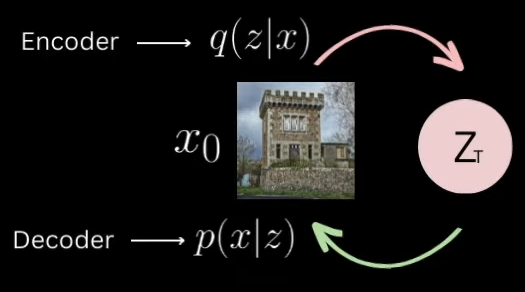
\includegraphics[width=0.5\textwidth]{fig/VAE.png}
    \caption{aproksimasi x pada VAE}
    \label{fig:aproksimasi_x_pada_VAE}
\end{figure}
Di sini, kita ingin neural network agar dapat mengaproksimasi probability dari p of $ \textbf{x} $ sehingga dapat generate gambar yang semirip mungkin dengan distribusi  $ \textbf{x} $ (training data). Untuk itu, kita akan memaksimalkan log-likelihood dari $ p $. Fungsi log dibutuhkan agar nilai likelihood tidak exploding (terlalu besar hingga tidak bisa disimpan komputer). Fungsi log bersifat monotonic sehingga memaksimalkan log-likelihood berarti juga memaksimalkan true likelihood.
\begin{flalign*}
& \log p(x) = \log \int p(x,z) \,dz. &\\
& \hspace{3.9em} = \log \int p(x,z) \frac{q(z|x)}{q(z|x)} \,dz &\\
& \hspace{3.9em} = \log \mathbb{E}_{q(z|x)} \left[ \frac{p(x,z)}{q(z|x)} \right] &
\end{flalign*}
Logaritma merupakan fungsi concave. Hal ini dapat dibuktikan karena turunan kedua dari logaritma adalah negatif. Oleh sebab itu, berlaku: $ \log \mathbb{E}_{q(z|x)} \left[ \frac{p(x,z)}{q(z|x)} \right] = \mathbb{E}_{q(z|x)} \left[ \log \frac{p(x,z)}{q(z|x)} \right] $, sehingga:
\begin{flalign*}
& \log p(x) \geq \mathbb{E}_{q(z|x)} \left[\log \frac{p(x,z)}{q(z|x)} \right] &
\end{flalign*}

Kita dapat menerapkan hal yang sama pada diffusion models. Perbedaannya, kita tidak ke $ Z_T $, tetapi melalui urutan latent variable dari $ x_1 $ ke $ x_T $. Kita juga tidak lagi mencari loss function, melainkan ekspektasi dari loss function.
\begin{figure}[h]
    \centering
    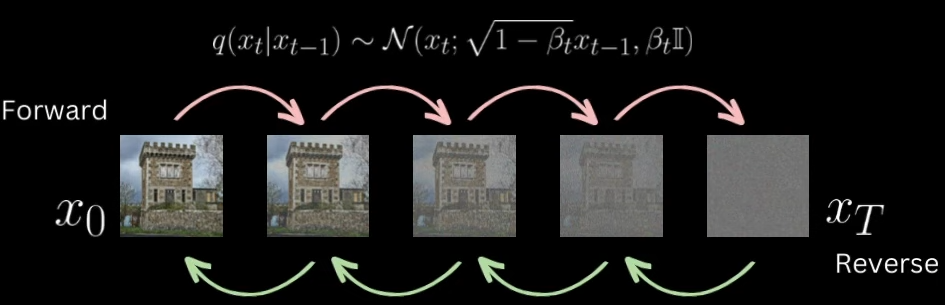
\includegraphics[width=0.5\textwidth]{fig/reverse-process.png}
    \caption{reverse process}
    \label{fig:reverse_process}
\end{figure}
Disamping itu, kita tidak memaksimalkan log-likelihood, melainkan meminimalkan negative log-likelihood. Sebenarnya, kedua hal tersebut sama. Namun, optimizer biasanya meminimalkan fungsi sehingga akan lebih cocok jika kita menggunakan negative log-likelihood. Seperti namanya, yaitu loss function, kita ingin meminimalkan fungsi ini sekecil mungkin.
\begin{flalign*}
& 
-\log p_\theta(\textbf{x}_0) 
= -\log \int p_\theta(\textbf{x}_{0:T}) \,d\textbf{x}_{1:T}. 
&\\
& \hspace{5.4em} = -\log \int p_\theta(\textbf{x}_{0:T}) \frac{q(\textbf{x}_{1:T}|\textbf{x}_0)}{q(\textbf{x}_{1:T}|\textbf{x}_0)} \,d\textbf{x}_{1:T} &\\
& \hspace{5.4em} = -\log \int q(\textbf{x}_{1:T}|\textbf{x}_0) \frac{p_\theta(\textbf{x}_{0:T})}{q(\textbf{x}_{1:T}|\textbf{x}_0)} \,d\textbf{x}_{1:T} &\\
& \hspace{5.4em} = -\log \mathbb{E}_{q(\textbf{x}_{1:T}|\textbf{x}_0)} \left[ \frac{p_\theta(\textbf{x}_{0:T})}{q(\textbf{x}_{1:T}|\textbf{x}_0)} \right] &\\
& \hspace{5.4em} \leq \mathbb{E}_{q(\textbf{x}_{1:T}|\textbf{x}_0)} \left[ -\log \frac{p_\theta(\textbf{x}_{0:T})}{q(\textbf{x}_{1:T}|\textbf{x}_0)} \right] &\\
& \hspace{5.4em} \leq \mathbb{E}_{q(\textbf{x}_{1:T}|\textbf{x}_0)} \left[ \log \frac{q(\textbf{x}_{1:T}|\textbf{x}_0)}{p_\theta(\textbf{x}_{0:T})} \right] &
\end{flalign*}

Selanjutnya, kita dapat melakukan optimasi pada term yang berada di dalam ekspektasi.
\begin{flalign*}
& \log \frac{q(\textbf{x}_{1:T}|\textbf{x}_0)}{p_\theta(\textbf{x}_{0:T})} = \log \frac{\displaystyle \prod_{t=1}^{T} q(\textbf{x}_{t}|\textbf{x}_{t-1})}{p(\textbf{x}_T) \displaystyle \prod_{t=1}^{T} p_\theta(\textbf{x}_{t-1}|\textbf{x}_{t})} &
\end{flalign*}

$ q(\textbf{x}_{t}|\textbf{x}_{t-1}) $ dapat kita ubah menjadi $ \frac{q(\textbf{x}_{t-1}|\textbf{x}_t) \ q(\textbf{x}_t) }{ q(\textbf{x}_{t-1}) } $. Namun, $ q(\textbf{x}_{t-1}|\textbf{x}_t) $ akan memiliki variance yang tinggi karena kandidat untuk $ \textbf{x}_{t} $ bisa bermacam-macam.
\begin{figure}[h]
    \centering
    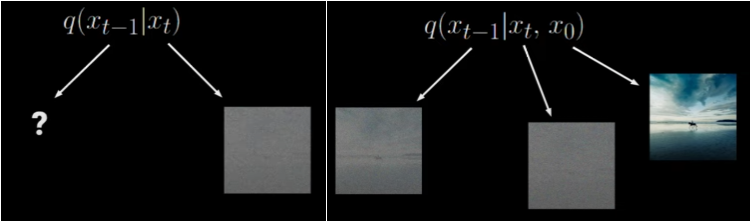
\includegraphics[width=0.75\textwidth]{fig/high-variance-vs-low-variance.png}
    \caption{high variance vs. low variance}
    \label{fig:high-variance-vs-low-variance}
\end{figure}

Oleh karena itu, kita akan menambahkan gambar asli $ \textbf{x}_0 $ agar kandidat untuk $ \textbf{x}_{t-1} $ dapat menyesuaikan gambar aslinya.
\begin{tabbing}
\hspace{6em} $ = \log \frac{\displaystyle \prod_{t=1}^{T} q(\textbf{x}_{t}|\textbf{x}_{t-1},\textbf{x}_0) } { p(\textbf{x}_T) \displaystyle \prod_{t=1}^{T} p_\theta(\textbf{x}_{t-1}|\textbf{x}_{t})} $
\end{tabbing}

Namun, terdapat hal yang janggal. Jika kita teliti lebih dalam, term pertama pada numerator mengandung self-loop! Lebih tepatnya, $ q(\textbf{x}_1|\textbf{x}_0,\textbf{x}_0) = \frac{q(\textbf{x}_0|\textbf{x}_1,\textbf{x}_0) \ q(\textbf{x}_1|\textbf{x}_0) }{ q(\textbf{x}_0|\textbf{x}_0) } $. Untuk mengatasi hal ini, keluarkan term pertama dari product series. Setelah itu, kita baru bisa menambahkan $ \textbf{x}_0 $ pada conditional probability di product series.
\begin{tabbing}
\hspace{6em} $ =\xcancel{ \log \frac{\displaystyle \prod_{t=1}^{T} q(\textbf{x}_{t}|\textbf{x}_{t-1},\textbf{x}_0) } { p(\textbf{x}_T) \displaystyle \prod_{t=1}^{T} p_\theta(\textbf{x}_{t-1}|\textbf{x}_{t})} } $\\\\

\hspace{6em} $ = \log \frac{q(\textbf{x}_1|\textbf{x}_0) \displaystyle \prod_{t=2}^{T} q(\textbf{x}_{t}|\textbf{x}_{t-1},\textbf{x}_0) } { p(\textbf{x}_T) \displaystyle \prod_{t=1}^{T} p_\theta(\textbf{x}_{t-1}|\textbf{x}_{t})} $\\\\

\hspace{6em} $ = \log \frac{q(\textbf{x}_1|\textbf{x}_0) \displaystyle \prod_{t=2}^{T} q(\textbf{x}_{t-1}|\textbf{x}_t,\textbf{x}_0) \ q(\textbf{x}_{t}|\textbf{x}_0) } { q(\textbf{x}_{t-1}|\textbf{x}_0) \ p(\textbf{x}_T) \displaystyle \prod_{t=1}^{T} p_\theta(\textbf{x}_{t-1}|\textbf{x}_{t})} $\\\\

\hspace{6em} $ = \log \frac{ 
\cancel{q(\textbf{x}_1|\textbf{x}_0)}
\ q(\textbf{x}_{T-1}|\textbf{x}_T,\textbf{x}_0) \ q(\textbf{x}_T|\textbf{x}_0) 
\ q(\textbf{x}_{T-2}|\textbf{x}_{T-1},\textbf{x}_0) \ \cancel{q(\textbf{x}_{T-1}|\textbf{x}_0)} 
\ ...
\ q(\textbf{x}_{1}|\textbf{x}_{2},\textbf{x}_0) \ \cancel{q(\textbf{x}_{2}|\textbf{x}_0)} 
} 
{ 
\cancel{q(\textbf{x}_{T-1}|\textbf{x}_0)} 
\ q(\textbf{x}_{T-2}|\textbf{x}_0)
\ ...
\ \cancel{q(\textbf{x}_{2}|\textbf{x}_0)}
\ \cancel{q(\textbf{x}_{1}|\textbf{x}_0)}
\ p(\textbf{x}_T) \displaystyle \prod_{t=1}^{T} p_\theta(\textbf{x}_{t-1}|\textbf{x}_{t}) } $\\\\

\hspace{6em} $ = \log \frac{
q(\textbf{x}_T|\textbf{x}_0) \displaystyle \prod_{t=2}^{T} q(\textbf{x}_{t-1}|\textbf{x}_t,\textbf{x}_0)
} 
{ 
p(\textbf{x}_T) \displaystyle \prod_{t=1}^{T} p_\theta(\textbf{x}_{t-1}|\textbf{x}_{t})
} $\\\\

\hspace{6em} $ = \log \frac{
q(\textbf{x}_T|\textbf{x}_0) \displaystyle \prod_{t=2}^{T} q(\textbf{x}_{t-1}|\textbf{x}_t,\textbf{x}_0)
} 
{ 
p(\textbf{x}_T) \ p_\theta(\textbf{x}_0|\textbf{x}_1) \displaystyle \prod_{t=2}^{T} p_\theta(\textbf{x}_{t-1}|\textbf{x}_{t})
} $\\\\

\hspace{6em} $ \displaystyle = \log \frac{
q(\textbf{x}_T|\textbf{x}_0)
} 
{ 
p(\textbf{x}_T)
} + 
\sum_{t=2}^{T} \log \frac{
q(\textbf{x}_{t-1}|\textbf{x}_t,\textbf{x}_0)
}
{
p_\theta(\textbf{x}_{t-1}|\textbf{x}_{t})
} -
\log p_\theta(\textbf{x}_0|\textbf{x}_1)
$
\end{tabbing}

Masukkan kembali $ \log \frac{q(\textbf{x}_{1:T}|\textbf{x}_0)}{p_\theta(\textbf{x}_{0:T})} $ pada loss function:
\begin{flalign*}
& -\log p_\theta(\textbf{x}_0) \leq \mathbb{E}_{q(\textbf{x}_{1:T}|\textbf{x}_0)} \left[ 
\log \frac{
q(\textbf{x}_T|\textbf{x}_0)
} 
{ 
p(\textbf{x}_T)
} + 
\sum_{t=2}^{T} \log \frac{
q(\textbf{x}_{t-1}|\textbf{x}_t,\textbf{x}_0)
}
{
p_\theta(\textbf{x}_{t-1}|\textbf{x}_{t})
} -
\log p_\theta(\textbf{x}_0|\textbf{x}_1)
\right]. &\\
\end{flalign*}

Ubah setiap term pada loss function ke bentuk KL (Kullback–Leibler divergence) divergence:
\begin{flalign*}
& 
\mathbb{E}_{q(\textbf{x}_{1:T}|\textbf{x}_0)} \left[ 
\log \frac{
q(\textbf{x}_T|\textbf{x}_0)
} 
{ 
p(\textbf{x}_T)
} + 
\sum_{t=2}^{T} \log \frac{
q(\textbf{x}_{t-1}|\textbf{x}_t,\textbf{x}_0)
}
{
p_\theta(\textbf{x}_{t-1}|\textbf{x}_{t})
} -
\log p_\theta(\textbf{x}_0|\textbf{x}_1)
\right] 
&\\
& 
\hspace{4em} = 
\mathbb{E}_{q(\textbf{x}_{1:T}|\textbf{x}_0)} \left[ 
\infdiv{q(\textbf{x}_T|\textbf{x}_0)}{p(\textbf{x}_T)}
+ 
\sum_{t=2}^{T} \infdiv{ 
q(\textbf{x}_{t-1}|\textbf{x}_t,\textbf{x}_0)
}
{
p_\theta(\textbf{x}_{t-1}|\textbf{x}_{t})
}
-
\log p_\theta(\textbf{x}_0|\textbf{x}_1)
\right]
&
\end{flalign*}

Didapatkan:
\\
\begin{equation}
{\small L = 
\mathbb{E}_{q} \left[ 
\infdiv{q(\textbf{x}_T|\textbf{x}_0)}{p(\textbf{x}_T)}
+ 
\sum_{t=2}^{T} \infdiv{ 
q(\textbf{x}_{t-1}|\textbf{x}_t,\textbf{x}_0)
}
{
p_\theta(\textbf{x}_{t-1}|\textbf{x}_{t})
}
-
\log p_\theta(\textbf{x}_0|\textbf{x}_1)
\right]
}
\end{equation}
\\
dengan 
\begin{equation}
q(\textbf{x}_{t-1}|\textbf{x}_t,\textbf{x}_0) = \mathscr{N}(\textbf{x}_{t-1};\tilde{\mu}_t(\textbf{x}_{t},\textbf{x}_0),\tilde{\beta}_t\textbf{I}), 
\end{equation}
\\
\begin{equation}
\tilde{\mu}_t(\textbf{x}_{t},\textbf{x}_0) \coloneq \frac{
\sqrt{\bar{\alpha}_{t-1}}\beta_t
}
{
1 - \bar{\alpha}_t
}
\textbf{x}_0 
+
\frac{
\sqrt{\alpha_{t}}(1-\bar{\alpha}_{t-1})
}
{
1 - \bar{\alpha_t}
}
\textbf{x}_t,
\end{equation}
\\
\begin{equation}
\tilde{\beta}_t \coloneq 
\frac{
1-\bar{\alpha}_{t-1}
}
{
1-\bar{\alpha}
}
\beta_t.
\end{equation}

Kita dapat menguraikan L menjadi:
\\
\begin{equation}
L_T = 
\infdiv{q(\textbf{x}_T|\textbf{x}_0)}{p(\textbf{x}_T)}.
\end{equation}
\\
\begin{equation}
L_{t-1} = 
\infdiv{ 
q(\textbf{x}_{t-1}|\textbf{x}_t,\textbf{x}_0)
}
{
p_\theta(\textbf{x}_{t-1}|\textbf{x}_{t})
}.
\end{equation}
\\
\begin{equation}
L_{0} = 
\log p_\theta(\textbf{x}_0|\textbf{x}_1).
\end{equation}
\\


\subsection{Forward process dan $ L_T $}
Sebenarnya, $ \beta_t $ dapat dipelajari melalui reparameterization. Namun, nilai $ \beta_t $ akan dibuat tetap menjadi konstanta sehingga q tidak ada parameter yang dapat dipelajari. Hal ini membuat $ L_T $ menjadi konstan selama training dan dapat diabaikan.


\subsection{Reverse process dan $ L_{1:T-1} $}
Kita ingin mempelajari mean dan variance dari reverse diffusion process $ p_\theta(\textbf{x}_{t-1}|\textbf{x}_{t}) = \mathscr{N}(\textbf{x}_{t-1};\mu_\theta(\textbf{x}_{t},t),\Sigma_\theta(\textbf{x}_t, t)) $, dengan $ 1 < t < T  $. Di sini, author memutuskan untuk tidak mempelajari variance dan menjadikannya konstanta:
\\
\begin{equation}
\Sigma_\theta(\textbf{x}_t, t) = \sigma_t^2 \textbf{I}
\end{equation}
\\
sehingga
\\
\begin{equation}
 p_\theta(\textbf{x}_{t-1}|\textbf{x}_{t}) = \mathscr{N}(\textbf{x}_{t-1};\mu_\theta(\textbf{x}_{t},t),\sigma_t^2 \textbf{I})
\end{equation}
\\

Untuk merepresentasikan mean $ \mu_\theta(\textbf{x}_{t},t) $, penulis DDPM melakukan parameterisasi berdasarkan analisis terhadap $ L_t $, yaitu $
\infdiv{ 
q(\textbf{x}_{t}|\textbf{x}_{t+1},\textbf{x}_0)
}
{
p_\theta(\textbf{x}_{t}|\textbf{x}_{t+1})
}
$, dengan menggunakan mean square error:
\begin{equation}
L_{t-1} = \mathbb{E}_{q} \left[ 
\frac{1}{2\sigma_t^2}
\norm{
\tilde{\mu}_t(\textbf{x}_{t},\textbf{x}_0) - \mu_\theta(\textbf{x}_{t},t)
}^2
\right] + C,
\end{equation}
dengan C adalah konstanta yang tidak bergantung pada $ \theta $. Subtitusi $ \tilde{\mu}_t(\textbf{x}_{t},\textbf{x}_0) $ pada (12):
\begin{flalign*}
L_{t-1} = \mathbb{E}_{q} \left[ 
\frac{1}{2\sigma_t^2}
\norm{
\frac{
\sqrt{\bar{\alpha}_{t-1}}\beta_t
}
{
1 - \bar{\alpha}_t
}
\textbf{x}_0 
+
\frac{
\sqrt{\alpha_{t}}(1-\bar{\alpha}_{t-1})
}
{
1 - \bar{\alpha_t}
}
\textbf{x}_t 
-
 \mu_\theta(\textbf{x}_{t},t)
}^2
\right] + C,
\end{flalign*}

Pada persamaan (2), kita telah diperlihatkan bagaimana mencari $ \textbf{x}_t $ jika diberikan $ \textbf{x}_0 $. Persamaan tersebut dapat kita gunakan untuk mencari $ \textbf{x}_0 $:
\begin{flalign*}
& \textbf{x}_t = \sqrt{\bar{\alpha_t}} \textbf{x}_{0} + \sqrt{1-\bar{\alpha_t}} \epsilon &\\
& \iff \textbf{x}_0 = \frac{1}{\sqrt{\bar{\alpha_t}}}(\textbf{x}_{t} - \sqrt{1-\bar{\alpha}_t} \epsilon) &
\end{flalign*}
Subtitusi $ \textbf{x}_0 $ pada (14):
\begin{flalign*}
&
L_{t-1} = \mathbb{E}_{q} \left[ 
\frac{1}{2\sigma_t^2}
\norm{
\frac{
\sqrt{\bar{\alpha}_{t-1}}\beta_t
}
{
1 - \bar{\alpha}_t
}
\frac{1}{\sqrt{\bar{\alpha_t}}}(\textbf{x}_{t} - \sqrt{1-\bar{\alpha}_t} \epsilon)
+
\frac{
\sqrt{\alpha_{t}}(1-\bar{\alpha}_{t-1})
}
{
1 - \bar{\alpha_t}
}
\textbf{x}_t 
-
\mu_\theta(\textbf{x}_{t},t)
}^2
\right] + C 
&\\
&
\hspace{2em} = \mathbb{E}_{q} \left[ 
\frac{1}{2\sigma_t^2}
\norm{
\frac{1}{\sqrt{\bar{\alpha}_t}}(\textbf{x}_t - \frac{\beta_t}{\sqrt{1-\bar{\alpha}_t}} \epsilon)
-
\mu_\theta(\textbf{x}_{t},t)
}^2
\right] + C 
&
\end{flalign*}

Penulis DDPM mereparameterisasi $ x_t $ agar dapat memprediksi noise pada reverse diffusion process:
\begin{equation}
\hspace{2em} = \mathbb{E}_{q} \left[ 
\frac{1}{2\sigma_t^2}
\norm{
\frac{1}{\sqrt{\bar{\alpha}_t}} ( \textbf{x}_t(\textbf{x}_0,\epsilon ) - \frac{\beta_t}{\sqrt{1-\bar{\alpha}_t}} \epsilon)
-
\mu_\theta(\textbf{x}_t(\textbf{x}_0,\epsilon),t)
}^2
\right] + C,
\end{equation}
dengan $ \textbf{x}_t(\textbf{x}_0,\epsilon) = \sqrt{\bar{\alpha}_t}\textbf{x}_0 + \sqrt{1-\bar{\alpha}_t}\epsilon, \hspace{1em} \epsilon \sim\mathscr{N}(0,\textbf{I}). $
Persamaan (10) memperlihatkan bahwa $ \mu_\theta $ harus memprediksi $ \frac{1}{\sqrt{\bar{\alpha}_t}} ( \textbf{x}_t(\textbf{x}_0,\epsilon ) - \frac{\beta_t}{\sqrt{1-\bar{\alpha}_t}} \epsilon) $, diberikan $ \textbf{t} $. Karena $ \textbf{t} $ sudah ada sebagai input, kita dapat melakukan parameterisasi sebagai berikut:
\begin{flalign*}
& \mu_\theta(\textbf{x}_{t},t) = \bar{\mu}_t(\textbf{x}_{t}, \textbf{x}_0(\textbf(x)_t, \epsilon_\theta)) &\\
& \hspace{2em} = \bar{\mu}_t(\textbf{x}_{t}, \frac{1}{\sqrt{\bar{\alpha_t}}}(\textbf{x}_{t} - \sqrt{1-\bar{\alpha}_t} \epsilon_\theta(\textbf{x}_t))) &
\end{flalign*}
\begin{fleqn}[\parindent]
\begin{equation}
\begin{split}
\hspace{2.25em} = \frac{1}{\sqrt{\bar{\alpha}_t}} ( \textbf{x}_t - \frac{\beta_t}{\sqrt{1-\bar{\alpha}_t}} \epsilon_\theta(\textbf{x}_t, t))
\end{split}
\end{equation}
\end{fleqn}

Subtitusi persamaan (16) pada persamaan (15):
\begin{flalign*}
& L_{t-1} = \mathbb{E}_{q} \left[ 
\frac{1}{2\sigma_t^2}
\norm{
\frac{1}{\sqrt{\bar{\alpha}_t}} ( \textbf{x}_t - \frac{\beta_t}{\sqrt{1-\bar{\alpha}_t}} \epsilon)
-
\mu_\theta(\textbf{x}_t,t)
}^2
\right] + C 
&\\
&
\hspace{2.25em} = \mathbb{E}_{q} \left[ 
\frac{1}{2\sigma_t^2}
\norm{
\frac{1}{\sqrt{\bar{\alpha}_t}} ( \textbf{x}_t - \frac{\beta_t}{\sqrt{1-\bar{\alpha}_t}} \epsilon)
-
\frac{1}{\sqrt{\bar{\alpha}_t}} ( \textbf{x}_t - \frac{\beta_t}{\sqrt{1-\bar{\alpha}_t}} \epsilon_\theta(\textbf{x}_t, t))
}^2
\right] + C 
&
\end{flalign*}
\begin{fleqn}[\parindent]
\begin{equation}
\begin{split}
\hspace{2.25em} = \mathbb{E}_{q} \left[ 
\frac{\beta_t^2}{2\sigma_t^2\alpha_t(1-\bar{\alpha}_t)}
\norm{
\epsilon
-
\epsilon_\theta(\textbf{x}_t, t)
}^2
\right] + C
\end{split}
\end{equation}
\end{fleqn}

Setelah melakukan percobaan, ternyata penulis DDPM berpendapat bahwa menghilangkan term pertama pada (17) pada proses training akan meningkatkan kualitas sample dan juga lebih mudah dalam implementasi:
\begin{equation}
L_{simple}(\theta) \coloneq \mathbb{E}_{q} \left[ 
\norm{
\epsilon
-
\epsilon_\theta(\textbf{x}_t, t)
}^2
\right]
\end{equation}

Recall $ p_\theta(\textbf{x}_{t-1}|\textbf{x}_{t}) = \mathscr{N}(\textbf{x}_{t-1};\mu_\theta(\textbf{x}_{t},t),\Sigma_\theta(\textbf{x}_t, t)) $, kita dapat mensample $ \textbf{x}_{t-1} $ melalui reparameterization trick $ \mathscr{N}(\mu,\sigma^2) = \mu + \sigma \epsilon $:
\begin{flalign*}
& \textbf{x}_{t-1} = \mu_\theta(\textbf{x}_{t},t) + \Sigma_\theta(\textbf{x}_{t},t) + \epsilon &
\end{flalign*}
\begin{fleqn}[\parindent]
\begin{equation}
\begin{split}
\hspace{2.25em} = \frac{1}{\sqrt{\bar{\alpha}_t}} ( \textbf{x}_t - \frac{\beta_t}{\sqrt{1-\bar{\alpha}_t}} \epsilon_\theta(\textbf{x}_t, t)) + \sqrt{\beta_t} \epsilon
\end{split}
\end{equation}
\end{fleqn}


\section{Data Scaling}


\end{document}